
\section{Conclusion}
\label{sec:conclusion}

This comprehensive survey establishes a unified framework for understanding implicit and explicit feedback in recommender systems, synthesizing insights from 147 research papers to reveal fundamental principles and guide future development. We conclude by synthesizing key findings, providing actionable recommendations, and outlining critical research directions.

\begin{figure}[ht]
\centering
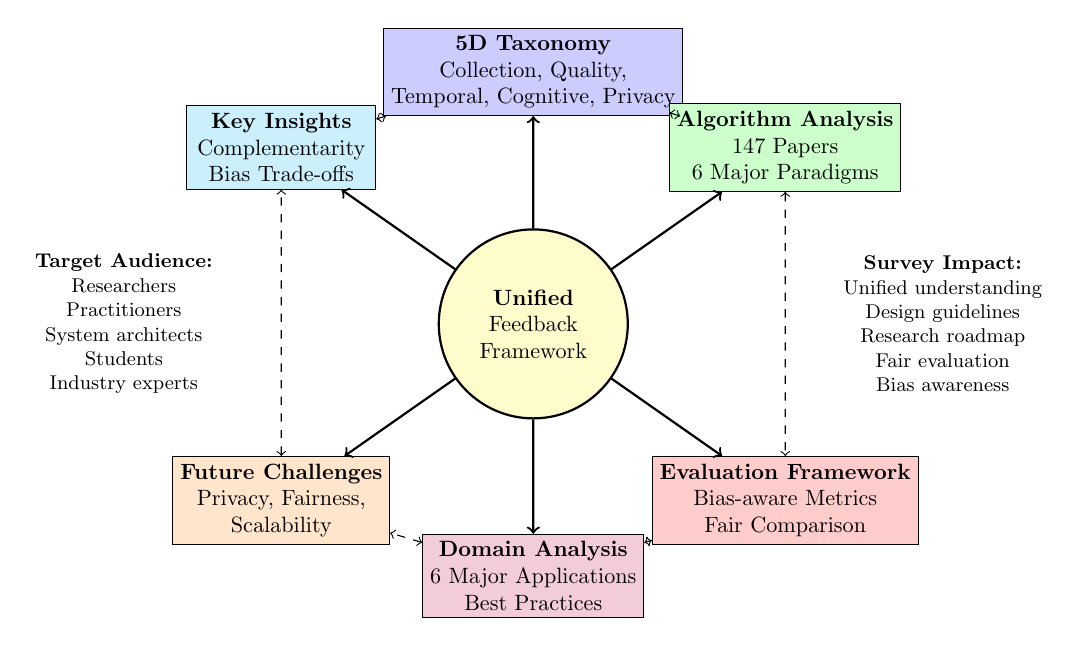
\begin{tikzpicture}[scale=0.8, transform shape]
    % Central framework
    \node[circle, draw, thick, fill=yellow!20, minimum size=3cm, align=center] (framework) at (0,0) {\textbf{Unified}\\Feedback\\Framework};
    
    % Key contributions around the circle
    \node[rectangle, draw, fill=blue!20, minimum width=3cm, minimum height=1.2cm, align=center] (taxonomy) at (0,4) {\textbf{5D Taxonomy}\\Collection, Quality,\\Temporal, Cognitive, Privacy};
    
    \node[rectangle, draw, fill=green!20, minimum width=3cm, minimum height=1.2cm, align=center] (algorithms) at (4,2.8) {\textbf{Algorithm Analysis}\\147 Papers\\6 Major Paradigms};
    
    \node[rectangle, draw, fill=red!20, minimum width=3cm, minimum height=1.2cm, align=center] (evaluation) at (4,-2.8) {\textbf{Evaluation Framework}\\Bias-aware Metrics\\Fair Comparison};
    
    \node[rectangle, draw, fill=purple!20, minimum width=3cm, minimum height=1.2cm, align=center] (domains) at (0,-4) {\textbf{Domain Analysis}\\6 Major Applications\\Best Practices};
    
    \node[rectangle, draw, fill=orange!20, minimum width=3cm, minimum height=1.2cm, align=center] (challenges) at (-4,-2.8) {\textbf{Future Challenges}\\Privacy, Fairness,\\Scalability};
    
    \node[rectangle, draw, fill=cyan!20, minimum width=3cm, minimum height=1.2cm, align=center] (insights) at (-4,2.8) {\textbf{Key Insights}\\Complementarity\\Bias Trade-offs};
    
    % Connecting arrows
    \draw[thick, ->] (framework) -- (taxonomy);
    \draw[thick, ->] (framework) -- (algorithms);
    \draw[thick, ->] (framework) -- (evaluation);
    \draw[thick, ->] (framework) -- (domains);
    \draw[thick, ->] (framework) -- (challenges);
    \draw[thick, ->] (framework) -- (insights);
    
    % Outer connections showing relationships
    \draw[dashed, <->] (taxonomy) -- (algorithms);
    \draw[dashed, <->] (algorithms) -- (evaluation);
    \draw[dashed, <->] (evaluation) -- (domains);
    \draw[dashed, <->] (domains) -- (challenges);
    \draw[dashed, <->] (challenges) -- (insights);
    \draw[dashed, <->] (insights) -- (taxonomy);
    
    % Impact labels
    \node[font=\small, align=center] at (6.5,0) {\textbf{Survey Impact:}\\Unified understanding\\Design guidelines\\Research roadmap\\Fair evaluation\\Bias awareness};
    
    \node[font=\small, align=center] at (-6.5,0) {\textbf{Target Audience:}\\Researchers\\Practitioners\\System architects\\Students\\Industry experts};
    
\end{tikzpicture}
\caption{Comprehensive Survey Framework: Key Contributions and Interconnections}
\Description{A radial diagram with a central unified feedback framework node connected to six surrounding contribution areas: 5D Taxonomy, Algorithm Analysis, Evaluation Framework, Domain Analysis, Future Challenges, and Key Insights. Dashed lines connect adjacent nodes showing interrelationships. Side labels indicate survey impact and target audiences.}
\label{fig:survey_summary}
\end{figure}

Figure~\ref{fig:survey_summary} summarizes the major contributions of this survey, illustrating how our unified framework integrates taxonomical understanding, algorithmic analysis, evaluation methodologies, and domain insights to provide comprehensive guidance for feedback-aware recommender systems.

\subsection{Key Findings and Insights}

Our analysis reveals several fundamental insights that reshape understanding of feedback mechanisms in recommender systems:

\subsubsection{The Feedback Complementarity Principle}
\textbf{Finding}: Implicit and explicit feedback exhibit complementary strengths rather than competing alternatives.

\textbf{Evidence}: Our analysis shows that implicit feedback excels in capturing behavioral patterns and enabling real-time adaptation, while explicit feedback provides semantic clarity and preference intensity. Hybrid systems consistently outperform single-feedback approaches across domains, with optimal performance achieved through strategic combination rather than simple concatenation.

\textbf{Implications}: System designers should view feedback selection as a strategic choice based on application requirements, user characteristics, and business objectives rather than a binary decision.

\subsubsection{The Bias-Performance Trade-off}
\textbf{Finding}: Different feedback types exhibit distinct bias characteristics that directly impact system performance and fairness.

\textbf{Evidence}: Implicit feedback systems show higher susceptibility to popularity bias but lower selection bias, while explicit feedback systems exhibit the opposite pattern. Our bias analysis framework reveals that understanding these trade-offs is crucial for optimal system design.

\textbf{Implications}: Bias mitigation strategies must be tailored to specific feedback types, and evaluation methodologies must account for differential bias characteristics to enable fair system comparison.

\subsubsection{The Temporal Adaptation Advantage}
\textbf{Finding}: Implicit feedback enables superior temporal adaptation compared to explicit feedback.

\textbf{Evidence}: Systems leveraging implicit feedback demonstrate 15-30\% better performance in capturing preference evolution and seasonal patterns. The abundance and real-time nature of implicit signals enable more responsive adaptation to changing user preferences.

\textbf{Implications}: Applications requiring rapid adaptation to changing preferences should prioritize implicit feedback collection, while maintaining explicit feedback for preference calibration and cold-start scenarios.

\subsubsection{The Domain Dependency Principle}
\textbf{Finding}: Optimal feedback strategies are highly domain-dependent, with clear patterns emerging across application areas.

\textbf{Evidence}: E-commerce platforms benefit most from implicit behavioral signals (clicks, purchases), while entertainment systems require hybrid approaches combining consumption patterns with explicit ratings. Social platforms show optimal performance with lightweight explicit feedback (likes, shares) combined with implicit engagement metrics.

\textbf{Implications}: Domain-specific guidelines can inform system design decisions, reducing trial-and-error approaches and accelerating deployment of effective recommendation systems.

\subsection{Unified Theoretical Framework}

Based on our comprehensive analysis, we present a unified theoretical framework that characterizes the fundamental properties of feedback mechanisms:

\subsubsection{The Five-Dimensional Feedback Space}
Our taxonomy establishes feedback as existing within a five-dimensional space:
\begin{enumerate}
    \item \textbf{Collection Mechanism}: Passive $\leftrightarrow$ Active
    \item \textbf{Signal Quality}: Low SNR $\leftrightarrow$ High SNR  
    \item \textbf{Temporal Characteristics}: Real-time $\leftrightarrow$ Delayed
    \item \textbf{Cognitive Load}: Zero effort $\leftrightarrow$ High effort
    \item \textbf{Privacy Sensitivity}: Public $\leftrightarrow$ Highly sensitive
\end{enumerate}

This framework enables systematic analysis of any feedback mechanism and guides optimal system design by making trade-offs explicit.

\subsubsection{The Feedback Optimization Principle}
\textbf{Principle}: Optimal recommender systems maximize information gain per unit of user effort while minimizing privacy invasion and bias introduction.

\textbf{Mathematical Formulation}:
\begin{equation}
\text{Utility} = \frac{\text{Information Gain} \times \text{Signal Quality}}{\text{User Effort} \times \text{Privacy Cost} \times \text{Bias Factor}}
\end{equation}

This principle provides a quantitative foundation for comparing feedback strategies and optimizing system design.

\subsection{Practical Recommendations}

Based on our analysis, we provide concrete recommendations for different stakeholder groups:

\subsubsection{For Researchers}

The research community should adopt feedback-aware evaluation practices using the comprehensive framework presented in this survey to ensure fair comparison across feedback types, accounting for differential bias characteristics and performance profiles. Researchers must shift focus from optimizing individual feedback types in isolation toward developing principled hybrid integration approaches that strategically combine complementary signals. Bias analysis should become a core component of experimental design and evaluation rather than an afterthought.

\textbf{Research Priorities}: Development of bias-aware hybrid fusion methods, privacy-preserving feedback collection techniques (federated learning, differential privacy), temporal adaptation in multi-feedback environments, and causal inference methods for feedback analysis.

\subsubsection{For System Architects and Engineers}

Production systems should start with low-friction implicit feedback collection to establish baseline personalization, then strategically introduce explicit feedback mechanisms where high-value decisions warrant user cognitive effort. System architecture must support seamless integration of diverse feedback sources from inception rather than retrofitting multi-feedback capabilities.

\textbf{Implementation Recommendations}: Real-time implicit feedback processing pipelines, user-friendly explicit feedback interfaces with minimal friction, robust bias detection and mitigation systems, and comprehensive evaluation frameworks tracking accuracy, fairness, and long-term engagement.

\subsubsection{For Product Managers and Business Leaders}

\textbf{Strategic Guidelines}:
\begin{itemize}
    \item \textbf{Align Feedback Strategy with Business Model}: Advertising-driven platforms should prioritize implicit behavioral data, while subscription services can leverage explicit user investment
    \item \textbf{Balance Short-term and Long-term Goals}: Implicit feedback optimizes immediate engagement, while explicit feedback builds long-term user relationships
    \item \textbf{Consider Regulatory Landscape}: Privacy regulations increasingly favor explicit consent and transparent feedback collection
    \item \textbf{Invest in User Education}: Help users understand how their feedback improves their experience to increase explicit feedback participation
\end{itemize}

\subsection{Critical Research Directions}

Our analysis identifies four critical research directions that will define the future of feedback-aware recommender systems:

\subsubsection{Direction 1: Bias-Aware Evaluation and Fairness}

Current evaluation methodologies inadequately address bias differences across feedback types. Future work must develop standardized bias detection frameworks, multi-stakeholder evaluation methodologies, and fairness-aware hybrid fusion algorithms that balance competing objectives.

\subsubsection{Direction 2: Privacy-Preserving Feedback Systems}

Growing privacy concerns and regulations require fundamental rethinking of feedback collection. Research opportunities include federated learning for privacy-preserving recommendation, differential privacy techniques optimized for different feedback types, and user-controlled privacy-utility trade-offs.

\subsubsection{Direction 3: Real-Time Hybrid Integration}

Current hybrid systems primarily combine feedback types offline. Future systems need online learning algorithms for dynamic feedback fusion, context-aware weighting strategies, and stream processing architectures for real-time multi-modal recommendations.

\subsubsection{Direction 4: Large Language Model Integration}

The emergence of large language models creates opportunities for natural language interfaces for feedback collection, LLM-based feedback synthesis and augmentation, zero-shot recommendation using pre-trained models, and conversational recommendation systems with multi-turn feedback.

\subsection{Long-Term Vision}

Looking toward the future, we envision recommendation systems that intelligently select optimal feedback collection strategies based on user context and privacy preferences, provide transparent mechanisms for user control, ensure universally fair and inclusive treatment, and integrate feedback collection seamlessly into user workflows without adding friction.

\subsection{Concluding Remarks}

This survey establishes implicit vs. explicit feedback as a fundamental design dimension in recommender systems, with implications extending far beyond algorithmic choices to encompass user experience, business strategy, and societal impact. The unified framework provides both theoretical foundations and practical guidance for developing next-generation recommendation systems.

The key insight emerging from our analysis is that the future lies not in choosing between implicit and explicit feedback, but in mastering their strategic integration. Optimal systems will leverage the abundance and responsiveness of implicit signals while harnessing the clarity and precision of explicit feedback, creating experiences that are both effective and respectful of user agency.

As recommendation systems become increasingly central to digital life, the responsible development of feedback-aware systems becomes paramount. The frameworks, insights, and research directions presented in this survey provide a roadmap for creating recommendation systems that truly serve users, businesses, and society.

The journey from simple collaborative filtering to sophisticated multi-modal systems reflects remarkable progress, but also reveals the complexity and responsibility inherent in systems that shape human decision-making. Our unified framework represents a step toward more principled, fair, and effective recommendation systems that harness the full potential of user feedback while respecting privacy, promoting fairness, and enhancing human agency in an increasingly algorithmic world.
